\section{Dynamic Programming}

    \frame{\sectionpage}

    \begin{frame}{0-1 Knapsack Problem}
        The most common problem being solved is the 0-1 knapsack problem, which restricts the number $ x_{i} $ of copies of each kind of item to zero or one. Given a set of $ n $ items numbered from 1 up to $ n $, each with a weight $ w_{i} $ and a value $ v_{i} $, along with a maximum weight capacity $ W $,
        \uncover<+->{\begin{equation*}
            \begin{align}
              \max& \sum _{i=1}^{n}v_{i}x_{i} \\
              \text{s.t.}& \sum _{i=1}^{n}w_{i}x_{i}\leq W $ \text{and} $ x_{i}\in \{0,1\}.
            \end{align}
            \end{equation*}}
    \end{frame}

    \begin{frame}{0-1 Knapsack Problem}
      \uncover<+>{Assume $ w_{1},\,w_{2},\,\ldots ,\,w_{n},\,W $ are strictly positive integers. Define $ m[i,w] $ to be the maximum value that can be attained with weight less than or equal to $ w $ using items up to $ i $.
      We can define $ m[i,w] $ recursively as follows:}

        \uncover<+>{
        \begin{equation*}
          \begin{align}
            m[0,\,w]&=0 \\
            m[i,\,w]&=m[i-1,\,w] ~\text{if}  ~w_{i}>w \\
            m[i,\,w]&=\max(m[i-1,\,w],\,m[i-1,w-w_{i}]+v_{i}) ~\text{if} ~w_{i} \leq w. \\
          \end{align}
        \end{equation*}}

    \end{frame}

    \begin{frame}{0-1 Knapsack Problem}
      \uncover<+->{The solution can then be found by calculating $ m[n,W] $. To do this efficiently, we can use a table to store previous computations.
      This solution will therefore run in $ O(nW) $ time and $ O(nW) $ space.}\\
      \vspace{6pt}
      \centering
      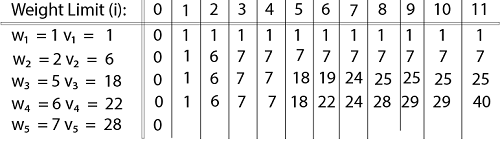
\includegraphics[width = 0.8\textwidth]{images/0-1-knapsack-problem1.png}
    \end{frame}

    \begin{frame}{Optimal substructure}
      \begin{itemize}
        \justifying
        \item Fibonacci sequence
        \begin{equation*}
          fib(n) = fib(n-1) + fib(n-2)
        \end{equation*}
        \item Dijkstra's algorithm for the shortest path problem
        \begin{equation*}
          d[y] = \min_x\{d[y], d[x]+w(x,y)\}
        \end{equation*}
      \end{itemize}
      How to define the status and stage of problems is essential.
    \end{frame}

    \begin{frame}{Shortest path problem}
        Given a directed graph $(V, A)$ with source node $s$, target node $t$, and cost $w_{ij}$  for each edge $(i, j)$ in $A$, consider the program with variables $x_{ij}$.
        \centering
        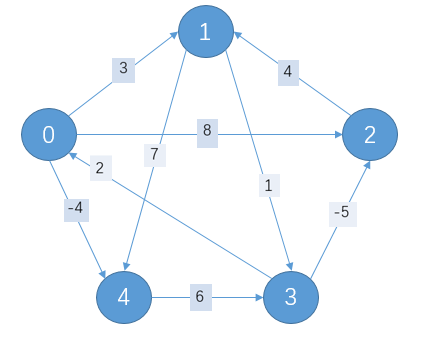
\includegraphics[width = 0.6\textwidth]{images/Shortest1.png}
    \end{frame}

    \begin{frame}{Shortest path problem}
      \begin{itemize}
        \item Integer programming formulation:
      \end{itemize}
      \begin{equation*}
        \begin{align}
        \min& \sum_{(i,j)\in A}w_{ij}x_{ij}\\
        \text{s.t.} &\sum_{j}x_{ij}-\sum_{j}x_{ji}={\begin{cases}1,&{\text{if }}i=s;\\-1,&{\text{if }}i=t;\\0,&{\text{ otherwise.}}\end{cases}}\\
        & x\in \{0,1\} ~\text{and for all} ~i.
        \end{align}
      \end{equation*}
    \end{frame}

    \begin{frame}{Shortest path problem}
      \begin{itemize}
        \item Find the shortest path from s to t.
        \centering
        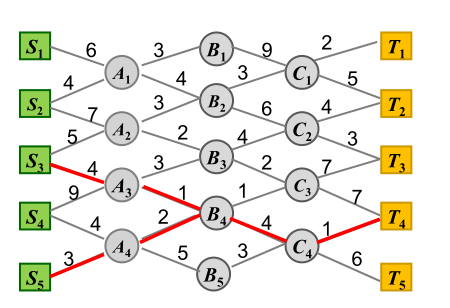
\includegraphics[width = 0.8\textwidth]{images/Shortest3.png}
      \end{itemize}
    \end{frame}

    \begin{frame}{Shortest path problem}
    \begin{spacing}{2}
    \begin{equation*}
      \begin{align}
    \textcolor{yellow}{Stage 1}\quad &F(C_l) = \min_m\{C_lT_m\} \\
    \textcolor{red}{Stage 2}\quad &F(B_k) = \min_l\{B_kC_l+F(C_l)\} \\
    \textcolor{blue}{Stage 3}\quad &F(A_j) = \min_k\{A_jB_k+F(B_k)\} \\
    \textcolor{green}{Stage 4}\quad &F(S_i) = \min_j\{S_iA_j+F(A_j)\}
      \end{align}
    \end{equation*}
    \end{spacing}
    \end{frame}

    \begin{frame}{Shortest path problem}
      \begin{itemize}
        \item Find the shortest path from s to t.
        \centering
        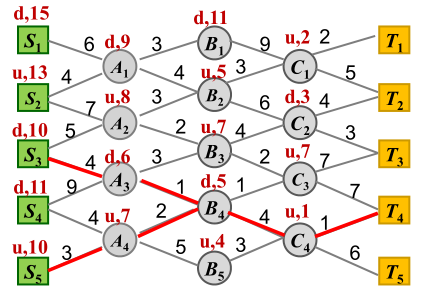
\includegraphics[width = 0.8\textwidth]{images/Shortest2.png}
      \end{itemize}
    \end{frame}
